\documentclass[10pt, A4]{article}
\usepackage[T1]{fontenc}
\usepackage{CJKutf8}
\usepackage[english]{babel}
\usepackage[utf8]{inputenc}

\usepackage{amsmath}
\usepackage{amssymb}
\usepackage{graphicx}
\usepackage{enumitem}
\graphicspath{ {./images/} }
 
\begin{CJK}{UTF8}{mj}

\title{Semi-Lagrangian과 PIC 방법을 사용한 그리드 기반 유체 애니메이션의 구현과 비교}
\author{장필식}
\date{2018. 12. 27}

\begin{document}

\maketitle

\begin{abstract}
\end{abstract}

\newpage

\tableofcontents

\newpage

\section{Introduction}

컴퓨터 그래픽스에서의 유체 시뮬레이션은 크게 두 접근방법으로 나뉘는데, 유체를 파티클의 집합으로 보아 각 파티클의 위치를 직접 시뮬레이션하는 Lagrangian 접근법, 그리고 유체를 유속의 vector field로 보아 파티클들이J 주어진 위치에서 유체가 지나가는 속도를 시뮬레이션하는 Eulerian Simulation이 있다. Semi-Lagrangian Method와 PIC Method 모두 양쪽 접근법을 같이 쓰는데, 이 연구에서는 이 둘을 구현한 다음에 서로 비교하여 장단점에 대해 알아볼 것이다.

\section{Methods}

본 섹션에서는 프로그램의 구현 방법에 대해서 설명할 것이다.

\subsection{Navier-Stokes Equation}

압축 불가능한 유체는 각 위치마다의 속도를 나타내는 vector field $\vec{u} : \mathbb{R}
^3 \rightarrow \mathbb{R}^3$ 나타낼 수 있는데, 다음과 같은 편미분방정식을 만족한다.

\begin{equation}
  \frac{\partial u}{\partial t} + \vec{u} \cdot \nabla{\vec{u}} + \frac{1}{\rho} \nabla{\vec{p}} = \vec{g} + \nu \nabla \cdot \nabla \vec{u}
\end{equation}

\begin{equation}
  \nabla \cdot \vec{u} = 0
\end{equation}

이 때 (1)은 Momentum Equation이고, (2)는 Imcompressibility condition이라고 명칭한다. 

이 편미분방정식을 한 번에 풀기에는 어려워, splitting이라는 방법을 통해 여러 개의 스텝으로 나눠서 풀게 된다.
간략하게 설명하자면, $\dot q = f(q) + g(q)$와 같은 미분방정식을 생각하자.
이것을 한 번에 푼다면 forward Euler를 사용해 $q = q_0 + \Delta t (f(q_0) + g(q_0))$로 구할 수 있다.
Splitting 방법은 $\dot q^a = f(q^a)$를 forward Euler 방법으로 먼저 푼 다음, 이 결과값을 사용해 $\dot q^b = f(q^b)$의 결과를 구하는 테크닉이다. 즉 $q'_0 = q_0 + \Delta t f(q_0)$, $q = q'_0 + \Delta t g(q'_0)$의 연산을 차례대로 하는 것이다. \cite[p.17-19]{fluid-sim-cg}

위의 테크닉을 사용해 편미분방정식 (1)을 다음과 같이 세 개의 식으로 분할할 수 있다.

\begin{equation}
  \frac{D\vec{q}}{Dt} = \frac{\partial \vec{q}}{\partial t} + \vec{q} \cdot \nabla \vec{q} = 0
\end{equation}
\begin{equation}
  \frac{\partial \vec{u}}{\partial t} = \vec{g}
\end{equation}
\begin{equation}
  \frac{\partial \vec{u}}{\partial t} + \frac{1}{\rho} \nabla p = 0
\end{equation}

이것을 가지고 최종적인 알고리즘을 만들어보자.
우리는 $\Delta t$의 시간간격을 가지고 $\vec{u}$를 불연속적으로 Integration을 수행할 것이다. 처음의 velocity field를 $\vec{u}^0$라고 하고, n번의 integration 수행 이후 (즉 $n \Delta t$의 시간 후)의 velocity field를 $\vec{u}^n$이라고 하자. (3), (5)의 편미분방정식을 푸는 함수를 \texttt{advect()}, \texttt{project()}라고 하면, $\vec{u}^n$에서부터 $\vec{u}^{n+1}$을 구하는 알고리즘은 다음과 같이 쓸 수 있다. \cite[p.20]{fluid-sim-cg}

\begin{align}
  \vec{u}^A &= advect(\vec{u}^n, \Delta t) \\
  \vec{u}^B &= \vec{u}^A + g \Delta t \\
  \vec{u}^{n+1} &= project(\vec{u}^B)
\end{align}

참고로 Incompressibility Condition ($\nabla \cdot \vec{u} = 0$)을 만족하게끔 하는 작업은 \texttt{project()} 함수에서 진행되는데, 이것에 대해서는 \textbf{Pressure Solve} 섹션에서 다룰 것이다.

\subsection{MAC Grid}

전 섹션에선는 시간을 연속에서 불연속적으로 변환했으므로, 여기서는 공간을 불연속적으로 변환하는 방법에 대해 설명할 것이다. 위치 공간 ($\mathbb{R}^3$)를 MAC Grid를 통해 불연속하게 쪼갤 것이다. \cite[p.21-25]{fluid-sim-cg}

시뮬레이션을 수행하는 영역을 $(i, j) \in [0, M \Delta x] \times [0, N \Delta x]$이라고 하자. 일반적인 2D Grid로 이 영역의 velocity field를 표현한다면, $i = 0..(M-1)$, $j = 0..(N-1)$에 대하여,  $(i \Delta x, j \Delta x)$의 위치마다 x축의 속도 $u(i, j)$, y축의 속도 $v(i, j)$를 저장하면 된다. 즉 크기 $(M, N)$의 2차원 어레이 2개를 저장하고 있으면 될 것이다. MAC Grid는 여기서 약간의 변형을 가하는데, 위치 $((i-1/2) \Delta x, j \Delta x)$ 마다 속도 $u(i-1/2, j)$, , 위치 $(i \Delta x, (j-1/2) \Delta x)$마다 속도 $v(i,j-1/2)$가 서로 Staggered된 형태로 아래의 그림과 같이 배치가 된다.

\begin{figure}[h]
\centering
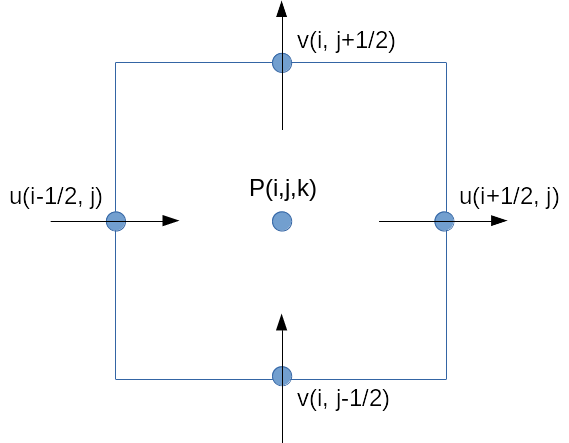
\includegraphics[width=0.5\textwidth]{mac_grid}
\caption{MAC Grid를 나태낸 그림}
\end{figure}

이젠 이것을 가지고 임의의 위치 $(x, y) \in \mathbb{R}^3$에서의 실제 속도값 $\vec{u}(x, y)$를 구할 수 있다. 예를 들어서 u에 대해서는 위치값이 1/2의 배수일 때 다음과 같이 구할 수 있다:

\begin{align*} 
  \vec{u}(i \Delta x, j \Delta x) &= (\frac{u(i-1/2, j) + u(i+1/2, j)}{2}, \frac{v(i,j+1/2) + v(i,j-1/2))}{2} \\
  \vec{u}((i+1/2) \Delta x, j \Delta x) &= (u(i,j), \frac{v(i,j-1/2) + v(i,j+1/2) + v(i+1,j-1/2) + v(i+1,j+1/2)}{4})
\end{align*}

임의의 위치에서의 Gradient 역시 쉽게 구할 수 있다:
\begin{align*}
  \vec{u}(i \Delta x, j \Delta x) &= (\frac{u(i+1/2, j) - u(i-1/2, j)}{\Delta x}, \frac{v(i,j+1/2) - v(i,j-1/2)}{\Delta x})
\end{align*}

위치값이 1/2의 배수로 떨어지지 않는 곳에서는 interpolation을 사용하여 값을 구할 수 있는데, 프로젝트에서는 bicubic interpolation을 사용한다.

\subsection{Advection: Semi-Lagrangian vs PIC method}

Semi-Lagrangian과 PIC Method (Particle-in-cell Method) 가 차이가 나는 부분은 주로 Advection Step에 있다. 

Semi-Lagrangian 방법에서는 Advection을 Eulerian 관점에서 접근해 그리드의 속도 값들에 대해 수행하게 된다. 만약에 순수히 Lagrangian 관점으로 Advection을 바라보면, i번째 particle의 현재 속력이 $\vec{v_i}$일때 위치 $\vec{x_i}$를 매 프레임마다 $\vec{x_i}(t + \Delta t) = \vec{x_i}(t) + \vec{v_i} \Delta t$로 integration을 해 주면 되므로 매우 간단하다. 하지만 Eulerian 관점에서는 속력에 대한 정보가 Grid에만 존재하므로 particle의 속력을 다른 방법을 사용해서 유추해야 한다. 그래서 Lagrangian 관점을 약간 차용해서, 시간 $t + \Delta t$에 어떠한 particle이 위치 $\vec{x}$를 지나갔다면, 그 particle은 시간 $t - \Delta t$에 위치 $\vec{x} - \vec{v} \Delta t$에 있을 것이라는 아이디어를 사용한다. 즉 $\Delta t$의 시간 뒤 위치 $\vec{x}$에서 속도는 위치 $\vec{x} - \vec{v} \Delta t$에서의 속도값으로 근사할 수 있다. (실제 프로그램의 구현에서는 $\vec{x} - \vec{v} \Delta t$와 같은 Forward-Euler가 아니라 3rd order Runge-Kutta Method를 사용한다.) \cite[p.29-33]{fluid-sim-cg}

Semi-Lagrangian 방법에서 Advection - Gravity - Pressure Solve 과정이 모두 끝난 후에는, Grid의 각 셀 값들을 유체인지, 혹은 빈 공간인지 업데이트해야 한다. 이것을 여러가지 방법으로 수행할 수 있는데, 가장 간단한 방법은 현재 유체인 셀들이 일정한 밀도로 marker particle들을 생성하고, 이 particle를 Pressure Solve에서 구한 velocity field를 사용해서 한 timestep동안 advection을 수행한 다음, 새로운 particle들의 위치를 가지고 level set을 만들어 유체 셀위 위치를 알아내는 방법이 있다. 조금 덜 번거로운 방법으로는 현재 유체의 영역을 나타내는 Level Set 자체에 advection을 수행하는 것이 있다 \cite[p.57]{fluid-sim-cg}. 프로그램의 구현에서는 전자의 방법을 수행한다.

Semi-Lagrangian에서는 실질적으로 Advection을 그리드에서 한번, 파티클들에서 한번 실행해야 한다는 단점이 있다. PIC Method는 이 두 가지 Advection을 하나로 통일화하는데, 시뮬레이션에서 파티클들의 위치와 속도 정보를 저장하여, advection step에서 파티클들을 직접 움직이는 방법이다. 이 방법의 문제ckdyd는 Advection 후에 Gravity/Pressure Solve 를 적용하려면 넘어갈려면 파티클의 속도값을 그리드로, 반대로 Gravity/Pressure Solve 후에 Advection을 적용하려면 그리드의 속도값을 파티클로 옮기는 작업이 필요하다. PIC는 interpolation을 사용해 Eulerian 관점과 Lagrangian 관점의 속도값을 서로 변환하게 된다. 

PIC Method에서 일어나는 interpolation은 값들을 smoothing하는 경향이 있어, 유체에 원하지 않는 viscosity를 가져오는 경향이 있다. 그래서 PIC에서 조금 수정을 가한 FLIP Method를 사용하기도 하는데, ... Bridson은 PIC와 FLIP을 $\alpha$만큼의 interpolation factor로 섞어서 쓰는것을 권장한다. 프로그램에서는 서로 다른 $\alpha$값을 가지고 실험해 볼 수 있는데, 이것이 유발하는 차이점에 대해서는 \textbf{Results} 셕션에서 다룰 것이다.

\subsection{Pressure Solve}

\textbf{MAC Grid} 섹션에서의 공식들을 사용해 (5)의 Pressure solve 공식을 다음과 같이 적용할 수 있다.

여기서 현재 유체의 상황을 반영하여 boundary condition을 주어야 하는데, 첫 번째는 비어있는 셀들에는 압력값이 0이라는 Dirichlet boundary condition이다 (특정 영역에 대해 가해지는 제한조건). 두 번째는 유체가 고체 벽을 통과하지 못한다는 것을 나타내는 Neumann boundary condition이다 (특정 면에 대해 가해지는 제한조건).

마지막 스텝인 Projection 스텝을 수행하기 위해서는 MICCG (Modified Incomplete Cholesky Conjugate Gradient) 방법을 사용한다. 이것은 선형 시스템을 푸는 대표적인 방법 중 하나인 Conjugate Gradient에 근사를 가해 좀 더 빠르게 만든 것으로, Bridson의 책 \cite[p.79]{fluid-sim-cg}에 잘 설명되어 있다.

\subsection{Level Set Method}

Pressure Solve 과정을 수행하는 데 중요한 부분 중에 하나가 어떤 위치에 유체 안쪽 혹은 바깥쪽에 있는지를 판별하는 것이다. 가장 간단하게 이것을 해결하는 방법은 파티클이 걸쳐있는 셀들을 모두 유체로 마킹하고 그렇지 않은 것은 빈 공간으로 마킹하는 것이다. 하지만 이 방법을 사용했을 때에는 파티클들의 수가 많지 않을 때 생기는 유체 내의 작은 기포 (빈 공간)를 매꾸지 못하여 유체의 내부에서 원하지 않는 유속이 생긴다는 문제를 발견하였다.

그래서 본 프로그램에서는 Level Set Method를 통해 signed distance function을 구하는 방법을 사용할 것이다. Signed distance function은 특정 지점에서 가장 가까운 유체 파티클까지의 거리를 나태낸다. (이름에 signed가 붙은 이유는 유체 내부에서는 음수가 되기 때문이다). 이 함수를 $\phi: \mathbb{R}^3 \rightarrow \mathbb{R}$이라고 하면, Eikonal equation ($|\nabla \phi| = 1$)를 만족하게 된다. 프로그램에서는 Closest Point Method \cite[p.11]{dist-function}로 유체 바깥과 경계의 $\phi$값들을 구한 다음, Fast Sweeping Method\cite{fast-sweeping}을 사용하여 유체 안쪽의 $\phi$값들도 구하게 된다. (자세한 방법은 \cite[p.49-p.56, p.126]{fluid-sim-cg} 참조.) Eikonal equation의 해 $\phi$를 찾아내고 나면, 특정 지점에서 $\phi$값이 음수인지 양수인지를 판별하여 유체의 안과 바깥을 구분한다.

프로그램에서 Level Set Method는 유체의 안과 바깥을 구분하는 것 이외에 다른 용도로도 쓰인다. Pressure solve를 진행할 때 빈 공간의 압력이 0이라는 Boundary Condition을 적용했는데, 이것은 유체의 경계에서 문제가 될 수 있다. Level-Set의 경계가 셀 사이를 지나가면서, 그리드에서 부분적으로만 채워져 있는 유체 셀들이 존재할 수 있기 때문에, 이 경우에는 이 셀들에 존재할 수 있는 압력에 대해 보정을 해 주어야 한다. 이것을 유체의 Level Set 함수를 사용해서 보정하는 방식이 Ghost Fluid Method인데, 이것을 사용하면 그리드로 인해 유체 시뮬레이션에서 생기는 artifact를 줄일 수 있다. \cite[p.127-129]{fluid-sim-cg}

\subsection{Summary}

즉 시뮬레이션의 메인 루프를 다음과 같이 쓸 수 있다:

\begin{verbatim}
loop:
  if (Semi-Lagrangian method):
    Create level set for fluid (and find fluid cells using the level set)
    Advect grid velocities using Semi-Lagrangian advection 
    Apply gravity to velocity field
    Solve for pressure and update velocity field
    Advect marker particles
  else if (PIC method):
    Create level set for fluid (and find fluid cells using the level set)
    Move velocities from particles to grid
    Apply gravity to velocity field
    Solve for pressure and update velocity field
    Move velocities from grid to particles
    Advect particles according to particle velocities
\end{verbatim}

\subsection{Implementation Details}

본 시뮬레이션은 C++로 구현하였으며, 여러 개의 코어에서 병렬화를 하기 위해 OpenMP를 사용하였다. (즉 OpenMP를 지원하는 컴파일러가 필요하다.) 프로그램 개발 환경은 Linux, 컴파일러는 Clang을 사용하였다. (코드는 https://github.com/lasagnaphil/fluid-sim에서 확인할 수 있다.) 개발에 사용된 라이브러리는 다음과 같다.

\begin{itemize}
  \item OpenGL (그래픽)
  \item SDL (창 생성/입출력 관련)
  \item IMGUI (UI 관련된 부분)
  \item MathFu (수학 라이브러리)
\end{itemize}

시뮬레이션의 성능을 높이기 위해서 여러가지 방법을 사용했는데, 일부 연산을 가속화시키기 위해 AVX/FMA SIMD intrinsics를 사용했다. (이것의 사용 유무를 CMake 빌드 세팅에서 \texttt{USE\_SIMD} 옵션으로 제어할 수 있다.) 예를 들어서, 연산에 많이 사용되는 함수 중 하나인 bicubic linear interpolation 함수, 그리고 pressure solve에서 자주 사용되는 벡터 간의 multiply-add 연산이 최적화 대상 중에 있었다.  그리고 OpenMP를 사용하여 유체 시뮬레이션 코드 중 병렬화가 편이한 부분 (loop index 사이에 dependency가 없는 for loop)을 여러 쓰레드에서 돌릴 수 있도록 했다.

사용자는 UI를 통해 중력의 크기 (x축과 y축)과 alpha값 (PIC/FLIP의 interpolation factor)를 바꿀 수 있고, 시뮬레이션에 관련된 중요한 값들 (현재 시간, 평균 압력, 평균 속도, CFL) 등을 볼 수 있다. 그리고 좌클릭 드래그를 통해 유체의 한 지점의 속도를 바꿀 수 있고, 우클릭 드래그를 통해 시뮬레이션 전체의 중력을 바꿀 수 있다.

\section{Results}

3가지의 초기 상태 (물 particle의 초기 위치) 에 대해서 시뮬레이션을 수행해 보있다.

\begin{enumerate}[label=\Alph*.]
  \item 모자 모양으로 되어 있는 배열 형태.
  \item 물 전체가 한쪽으로 기울어져 있는 형태.
  \item 정육면체의 모양의 물 영역이 떨어지는 형태.
\end{enumerate}

각각의 초기 상태에 대한 스크린샷은 다음과 같다.

\begin{figure}[h]
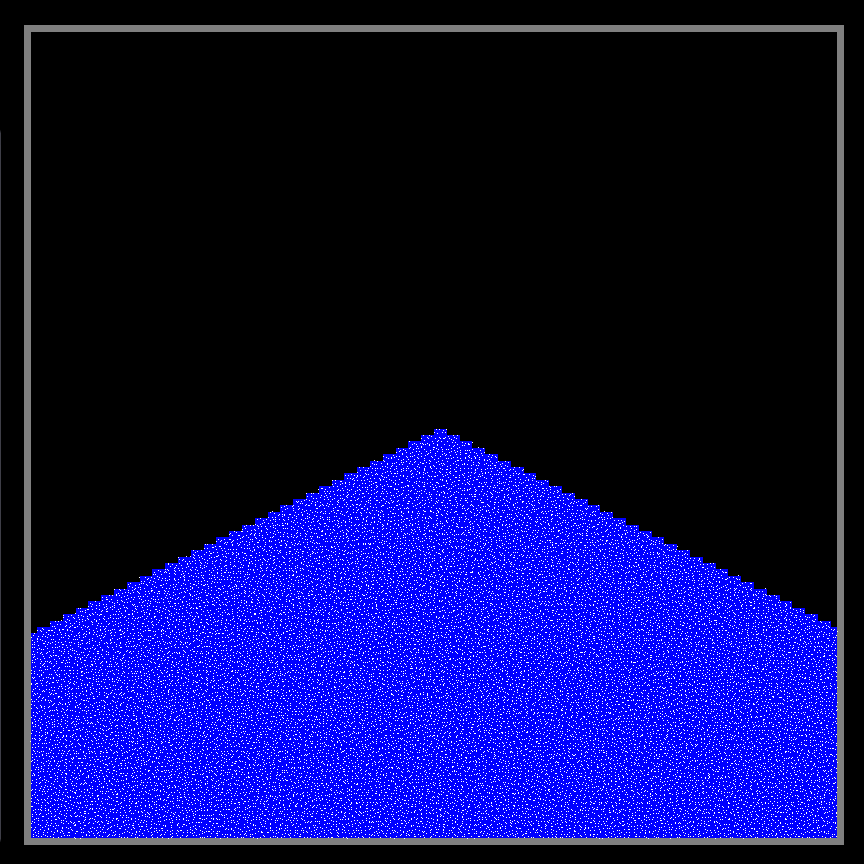
\includegraphics[width=0.32\textwidth]{init_state_1}
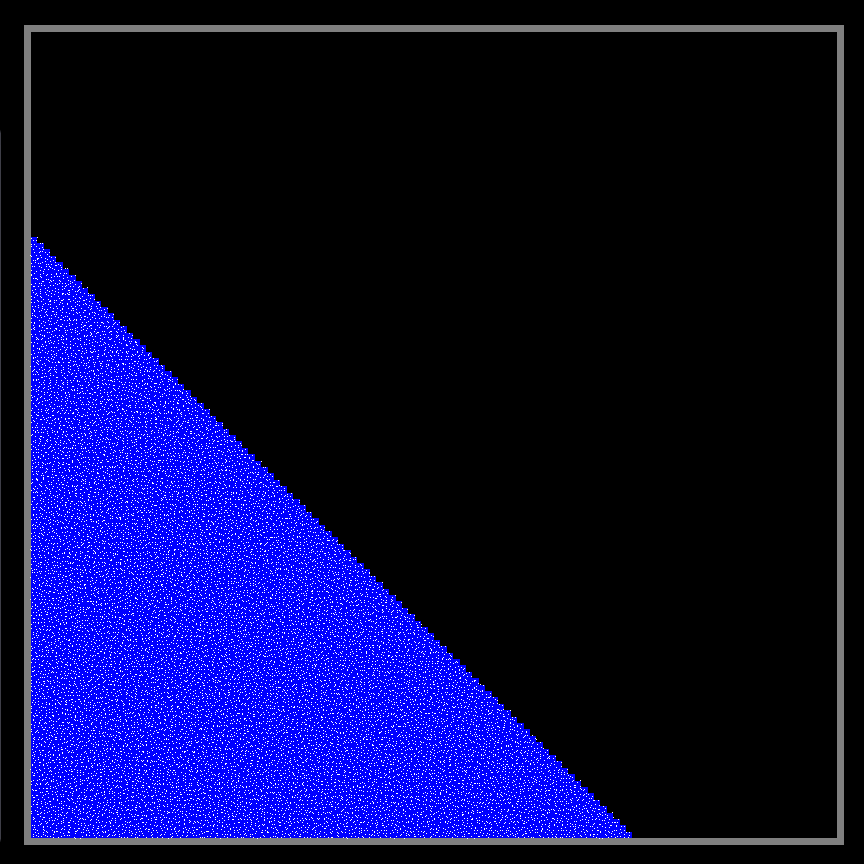
\includegraphics[width=0.32\textwidth]{init_state_2}
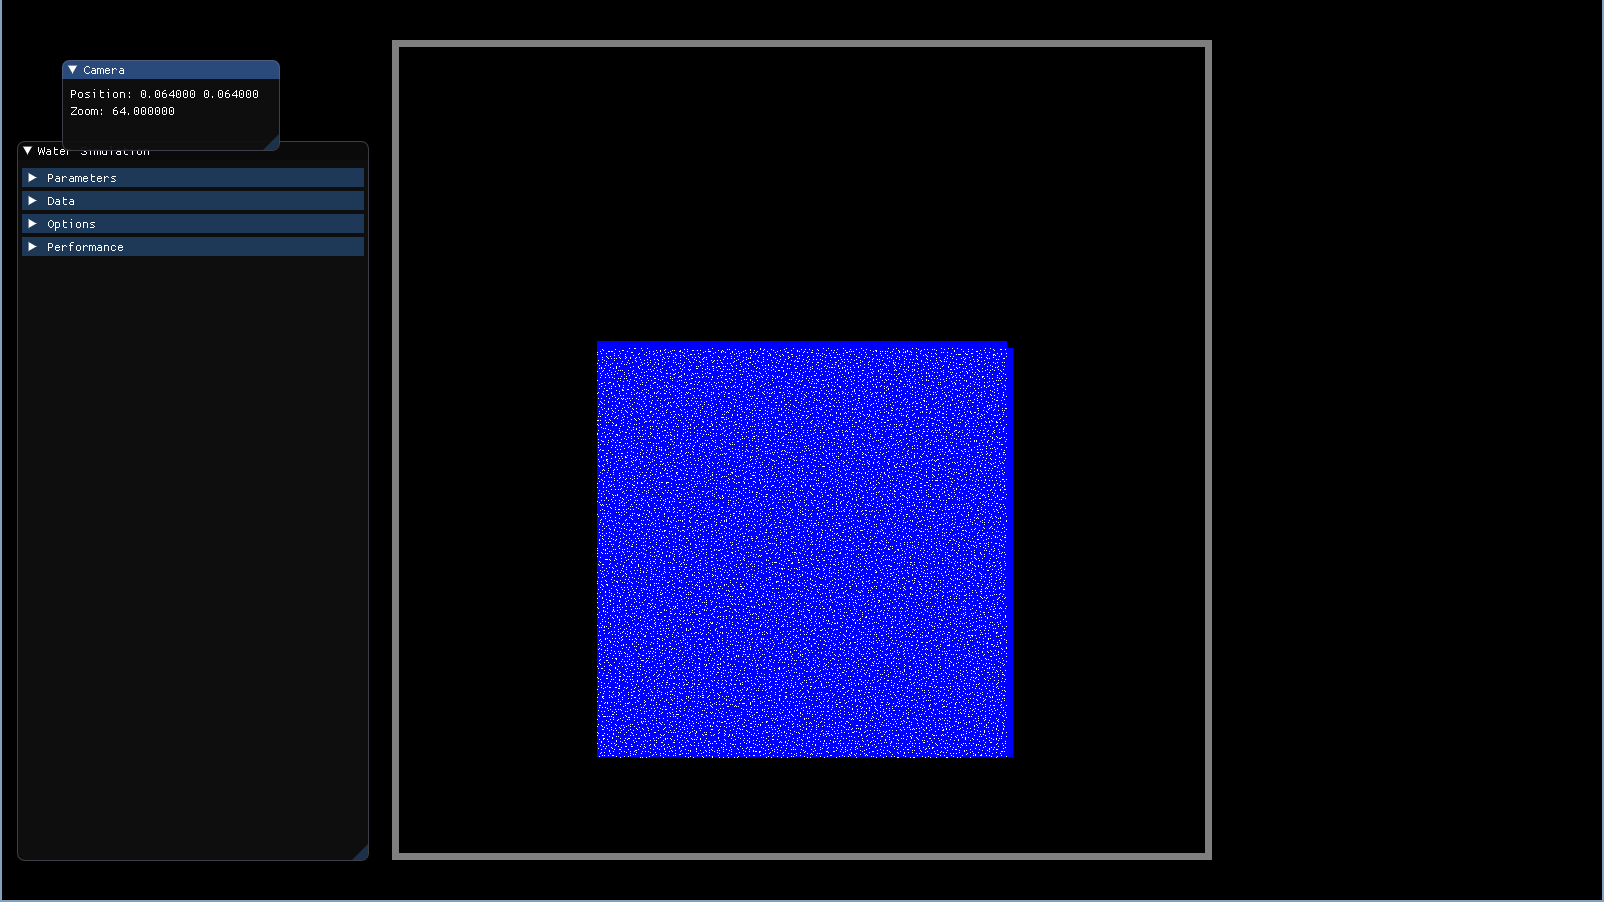
\includegraphics[width=0.32\textwidth]{init_state_3}
  \caption{3가지의 초기 상태를 나타낸 사진.}
\end{figure}

물의 움직임에 대한 동영상은 따로 링크로 첨부한다. (링크)

좌우로 진동하는 가속도 (진폭 3$m/s^2$, 주기 1.0s)를 주었을 때의 물의 운동을 관찰해 보았다. (Grid Size는 128x128, $\Delta x = 0.001m$, $\Delta t = 0.005s$)

\subsection{Realism}

PIC 방법이 Semi-Lagrangian 방법에 비해 좀 더 생동감 있는 모습을 보였다.

(예시 스크린샷 첨부)

눈으로만 보아서는 유체의 현실성을 평가하기 어렵기 때문에, 이론적으로 유체가 보존해야 하는 물리량들이 시간에 따라 어떻게 바뀌는지를 알아볼 것이다. 

그리고 PIC Method에서는 PIC와 FLIP의 Interpolation factor $\alpha$를 바꿔가면서 시뮬레이션을 수행하였다.

\begin{figure}[h]
  \centering
  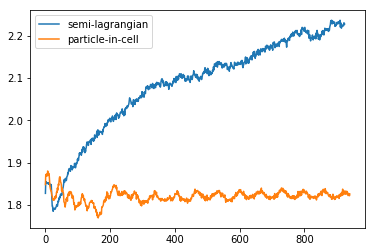
\includegraphics[width=0.7\textwidth]{picflip-volume-graph}
  \caption{PIC Method에서 시간에 따른 부피의 변화. alpha는 PIC/FLIP 사이의 interpolation factor이다.}
\end{figure}

위의 그래프를 분석하면 alpha값이 작아질수록 (즉 PIC보다 FLIP가 비중이 많아질수록) 부피가 원래보다 더욱 많이 팽창한다는 것을 알 수 있다. (예외라면 alpha=0.9일때 부피가 원래보다 감소하는 경향을 갖는다.) PIC만 사용하고 FLIP를 사용하지 않았을 때 (alpha = 1.0) 부피 보존이 가장 잘 됨을 확인할 수 있다.

\begin{figure}[h]
  \centering
  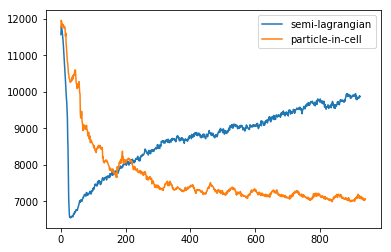
\includegraphics[width=0.7\textwidth]{picflip-energy-graph}
  \caption{PIC Method에서 시간에 따른 에너지의 변화. alpha는 PIC/FLIP 사이의 interpolation factor이다. 여기서 에너지는 Grid의 유체 Cell들의 에너지를 합한 결과이다.}
\end{figure}

\begin{figure}[h]
  \centering
  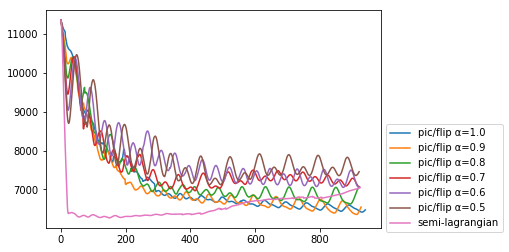
\includegraphics[width=0.7\textwidth]{picflip-particle-energy-graph}
  \caption{PIC Method에서 시간에 따른 에너지의 변화. alpha는 PIC/FLIP 사이의 interpolation factor이다. 여기서 에너지는 유체 Particle들의 에너지를 합한 결과이다.}
\end{figure}

(시간에 따른 부피 그래프 첨부)


\subsection{Stability}

Semi-Lagrangian이 좀 더 stable한 결과를 낼 수 있었다.

Stability의 예시: Semi-Lagrangian과 PIC를 같은 조건 (진동하는 가속도 진폭 X$m/s^2$, 주기 Xs) 에서 돌렸을 때 Semi-Lagrangian은 계속 구동했고 PIC는 Pressure Solve에서 터짐.
 
\subsection{Performance}

결과적으로는 128x128의 그리드 크기에 대해 노트북 CPU에서도 실시간으로 (30FPS 이상) 돌아가는 유체 시뮬레이션을 수행할 수 있었다. 아래는 Semi-Lagrangian과 PIC Method의 성능을 각각 다른 초기 조건 (A, B, C)에서 측정한 결과이다. 

\begin{table}[h]
\centering
\begin{tabular}{|l|l|l|l|l|}
\hline
                & A     & B     & C     & Average \\ \hline
Semi-Lagrangian & 31.32 & 27.32 & 26.51 & 28.38   \\ \hline
PIC/FLIP        & 24.57 & 20.91 & 19.09 & 21.52   \\ \hline
\end{tabular}
  \caption{초기 상태 A, B, C에서 각각 Semi-Lagrangian과 PIC Method를 사용했을 때의 한 프레임당 시뮬레이션 연산 시간 (단위는 ms. 조건: \Delta t = 0.033, \Delta x = 0.02, 그리드 크기는 128x128.)}
\end{table}

참고: 본 성능측정은 Intel(R) Core(TM) i7-6700HQ CPU (Quad core, Hyperthreading, 2.60Ghz)에서 진행했으며, 처음 30초 동안 프로그램을 돌렸을 때의 한 프레임 당 유체 시뮬레이션 코드가 걸린 전체 시간의 평균을 구한 것이다.

결과적으로 Semi-Lagrangian이 PIC/FLIP보다 연산시간이 많이 걸렸는데, 이것의 이유로는 Semi-Lagrangian 방법의 Advection Step에서 3rd order Runge-Kutta를 사용했는데, 이것을 수행하려면 한 셀당 bicubic interpolation을 총 6번 수행해야 했기 때문이다. 반면에 PIC/FLIP method에서는 Runge-Kutta 대신에 grid-to-particle, particle-to-grid transfer를 수행해야 했는데, 이 때는 bilinear sampling을 사용해서 연산량이 비교적 덜 소모되었다. (수치로 확인하면 Semi-Lagrangian advection은 0.922ms, grid-to-particle와 particle-to-grid transfer는 각각 0.447ms이 걸렸다.) 이것 이외에도 PIC Method가 Semi-Lagrangian Method의 Pressure Update 이 각각 4.41ms과 3.68ms가 걸려, PIC/FLIP에서 MICCG 알고리즘이 좀 더 빨리 수렴한다는 것을 알 수 있다.

\section{Discussion}

\subsection{Explanation of Results}

TODO

- 현실성/안정성 차이에 대한 설명

- 성능 차이에 대한 설명

\subsection{Further Improvements}

현재의 유체 시뮬레이션에서 가장 시급하게 해결해야 하는 것이 있다면, Pressure Solver의 numerical stability를 개선하는 것이다. 파티클의 속도가 굉장히 높아지는 극단적인 경우에 대해 Pressure Solver가 수렴을 하지 못해 올바른 해를 찾지 못하는 경우가 관찰되었는데, 실제로 산업에서 활용할 만한 기술로 만든다면 다양한 상황에 대해서도 무리 없이 돌아가도록 고쳐야 할 것이다. 이를 해결할 수 있는 방법 중 하나는 특정 파티클들의 속도가 너무 빨라지면 해당되는 파티클의 integration을 하는 timestep의 크기를 유동적으로 줄이는 것이다. \cite[p. 35]{fluid-sim-cg} 또 다른 해결 방안은 MICCG의 두 패러미터 값 $\tau$, $\sigma$를 조절해 보면서 더욱 좋은 수치를 찾는 것이다.

그리고 Semi-Lagrangian 방법과 PIC Method 모두 부피가 줄어드는 현상을 관찰할 수 있었는데, 이것은 특정 cell들에서 파티클의 밀도가 감소했기 때문으로 추정한다. 즉 이것을 해결하려면 파티클이 부족한 셀에 새로운 파티클을 추가하고, 파티클이 너무 많은 셀에 파티클을 제거하는 reseeding stage를 추가하면 해결 가능할 것으로 예상한다. (물론 reseeding에서 파티클의 수는 일정하게 유지되게 해야 한다.) 혹은 Kim et al. \cite{volume-preservation} 의 논문의 방법처럼 projection step에서 velocity field의 divergence를 0이 아닌 다른 값으로 보정해 해결하는 방식도 있다.

이것 외에도 PIC와 FLIP을 더욱 개선할 수 있는 APIC (Affine Particle-in-cell) 방법이 있는데, PIC에서의 dissipation이 일어나는 현상과 FLIP의 불안정성을 동시에 해결할 수 있는 방법이다. \cite{apic}

\section{Conclusion}

\begin{thebibliography}{9}
\bibitem{fluid-sim-cg}
Robert Bridson.
\textit{Fluid Simulation for Computer Graphics, Second Edition}. 
A K Peters/CRC Press, 2015.

\bibitem{dist-function}
Yen-hsi Richard Tsai,
\textit{Rapid and Accurate Computation of the Distance Function Using Grids}
Journal of Computational Physics, Volume 178, Issue 1, p. 175-195, 2002.

\bibitem{fast-sweeping}
Zhao, Hongkai.
\textit{A fast sweeping method for Eikonal equations}.
Mathematics of Computation, 74 (250): p. 603–627, 2005.

\bibitem{flip-fluids}
J.U.Brackbill, D.B.Kothe, H.M.Ruppel.
\textit{FLIP: A Low-dissipation, Particle-in-cell Method for Fluid Flow}.
Computer Physics Communications, 48, p. 25-38, 1988.

\bibitem{volume-preservation}
Kim, Byungmoon and Liu, Yingjie and Llamas, Ignacio and Jiao, Xiangmin and Rossignac, Jarek
\textit{Simulation of Bubbles in Foam with the Volume Control Method}
ACM Trans. Graph., 26.3, 2007.

\bibitem{apic}
Chenfanfu Jiang, Craig Schroeder, Andrew Selle, Joseph Teran, and Alexey Stomakhin.
\textit{The affine particle-in-cell method}.
ACM Trans. Graph., 34.4, Article 51, 2015.
\end{thebibliography}

\end{CJK}

\end{document}
